% ============================================================================
% Deep Surrogates to Estimate Dynamic Models
% Summer School on AI for Economics and Finance
% University of Padova, 23-24 September 2026
% Duration: 50 minutes
% ============================================================================

\documentclass[aspectratio=169,11pt]{beamer}

% ---------- Theme and colors ----------
\usecolortheme{dove}
\setbeamertemplate{navigation symbols}{}
\setbeamertemplate{footline}{%
  \hfill\usebeamerfont{page number in head/foot}%
  \usebeamercolor[fg]{normal text}%
  \insertframenumber\,/\,\inserttotalframenumber\kern1em\vskip4pt}
\setbeamerfont{frametitle}{size=\huge}

% ---------- Packages ----------
\usepackage[utf8]{inputenc}
\usepackage[T1]{fontenc}
\usepackage{amsmath,amssymb,amsfonts}
\usepackage{bm}
\usepackage{graphicx}
\usepackage{tikz}
\usetikzlibrary{shapes,arrows.meta,positioning,calc,fit,backgrounds,patterns,decorations.pathreplacing}
\usepackage{pgfplots}
\pgfplotsset{compat=1.18}
% --- readable-from-the-back defaults for every plot ---
\pgfplotsset{every axis/.append style={
    tick label style={font=\footnotesize},
    label style={font=\small},
    title style={font=\small},
    legend style={font=\footnotesize}}}
\usepgfplotslibrary{fillbetween}
\usepackage{booktabs}
\usepackage{hyperref}
\usepackage{multicol}
\usepackage{xcolor}
\usepackage{algorithmic}
\usepackage{listings}
\usepackage{pifont}
\usepackage{array}
\newcommand{\yes}{\textcolor{darkgreen}{\ding{51}}}
\newcommand{\no}{\textcolor{harvardcrimson}{\ding{55}}}
\newcommand{\mixed}{\textcolor{softorange}{\ding{108}}}

% ---------- Tighter display math, applied uniformly at every font size ------
% (a global typographic setting, so that no frame needs a local \vspace hack)
\makeatletter
\g@addto@macro\normalsize{%
  \setlength\abovedisplayskip{5pt plus 2pt minus 2pt}%
  \setlength\belowdisplayskip{5pt plus 2pt minus 2pt}%
  \setlength\abovedisplayshortskip{2pt plus 1pt}%
  \setlength\belowdisplayshortskip{3pt plus 1pt}}
\g@addto@macro\small{%
  \setlength\abovedisplayskip{4pt plus 2pt minus 2pt}%
  \setlength\belowdisplayskip{4pt plus 2pt minus 2pt}%
  \setlength\abovedisplayshortskip{2pt plus 1pt}%
  \setlength\belowdisplayshortskip{2pt plus 1pt}}
\g@addto@macro\footnotesize{%
  \setlength\abovedisplayskip{3pt plus 2pt minus 2pt}%
  \setlength\belowdisplayskip{3pt plus 2pt minus 2pt}%
  \setlength\abovedisplayshortskip{1pt plus 1pt}%
  \setlength\belowdisplayshortskip{2pt plus 1pt}}
\makeatother

% ---------- Custom colors ----------
\definecolor{uzhblue}{rgb}{0,0,0.5}
\definecolor{uzhgreylight}{RGB}{236,238,241}
\definecolor{uzhgreydark}{RGB}{81,86,94}
\definecolor{harvardcrimson}{RGB}{153,0,0}
\definecolor{unil@blue}{RGB}{0,140,204}
\definecolor{unil@black}{RGB}{35,31,32}
\definecolor{darkgreen}{RGB}{0,100,0}
\definecolor{darkred}{RGB}{139,0,0}
\definecolor{softblue}{RGB}{70,130,180}
\definecolor{softorange}{RGB}{230,159,0}
\definecolor{softgreen}{RGB}{0,158,115}

% ---------- Listings (after the colors it references) ----------
\lstset{
  language=Python,
  basicstyle=\small\ttfamily,
  keywordstyle=\color{uzhblue}\bfseries,
  commentstyle=\color{uzhgreydark}\itshape,
  stringstyle=\color{darkgreen},
  showstringspaces=false,
  breaklines=true,
  frame=none,
  aboveskip=2pt, belowskip=2pt}

% ---------- Set beamer colors ----------
\setbeamercolor{frametitle}{bg=uzhgreylight, fg=uzhblue}
\setbeamercolor{title}{fg=uzhblue}
\setbeamercolor{structure}{fg=uzhblue}
\setbeamercolor{block title}{bg=unil@blue, fg=white}
\setbeamercolor{block body}{bg=uzhgreylight}
\setbeamercolor{block title alerted}{bg=darkred,fg=white}
\setbeamercolor{block body alerted}{bg=red!5}
\setbeamercolor{block title example}{bg=darkgreen,fg=white}
\setbeamercolor{block body example}{bg=green!5}
\setbeamercolor{item}{fg=unil@black}
\setbeamercolor{normal text}{fg=unil@black}

% ---------- Emphasis and hyperlinks ----------
\newcommand{\emphc}[1]{\textcolor{harvardcrimson}{#1}}
\hypersetup{colorlinks,linkcolor=harvardcrimson,urlcolor=harvardcrimson}

% ---------- Finger-exercise badge ----------
\newcommand{\exercisepause}{%
  \tikz[baseline=(XB.base)]{%
    \node[rectangle, rounded corners=2pt, fill=softgreen!25, draw=softgreen!70!black,
          inner xsep=4pt, inner ysep=1.5pt,
          font=\footnotesize\bfseries, text=darkgreen] (XB) {PAUSE: 5 min};}}

% ---------- Math commands ----------
% One symbol, one meaning. See the notation frame in Part I.
% NOTE: this lecture is an estimation/policy lecture, so theta is the STRUCTURAL
% parameter vector, not the network weights (which the morning deck called theta).
\newcommand{\x}{\bm{x}}
\newcommand{\R}{\mathbb{R}}
\newcommand{\E}[1]{\mathbb{E}\!\left[#1\right]}
\newcommand{\str}{\bm{\theta}}          % structural parameters
\newcommand{\pol}{\bm{\vartheta}}       % policy parameters
\newcommand{\netw}{\bm{w}}              % network weights
\newcommand{\surr}{\phi}                % the surrogate
\DeclareMathOperator*{\argmin}{arg\,min}
\DeclareMathOperator*{\argmax}{arg\,max}

% ---------- Title ----------
\title[Surrogates -- Padova 2026]%
{Deep Learning for Solving Dynamic Models}
\subtitle{Session 6: Deep surrogates and Gaussian processes}
\author{Simon Scheidegger}
\institute[HEC Lausanne]{HEC, University of Lausanne\\[4pt]
{\footnotesize Based on Chen, Didisheim \& Scheidegger (2026), \emph{Journal of Financial Economics} 177, 104222}}
\date{University of Padova\\September 24, 2026}

\begin{document}

% ============================================================================
% PART 0: TITLE & OUTLINE
% ============================================================================

{\setbeamercolor{background canvas}{bg=uzhgreylight}
\begin{frame}
\titlepage
\end{frame}
}

\begin{frame}{Day 2 at a Glance}
\begin{center}
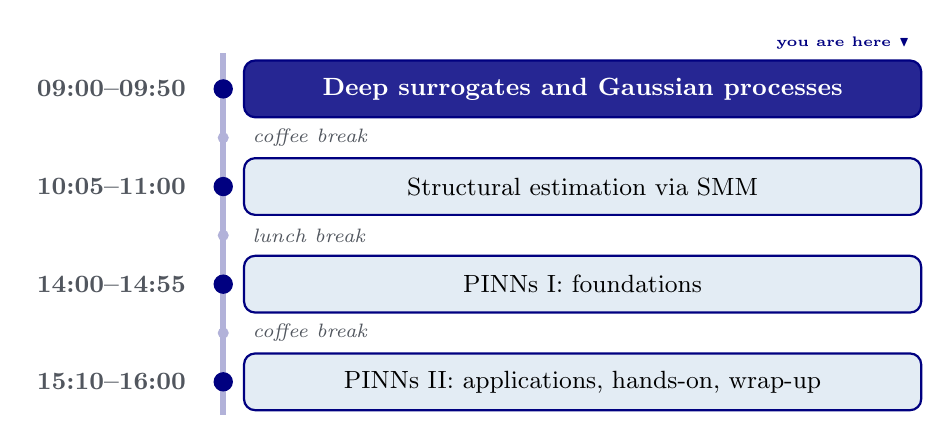
\begin{tikzpicture}[
    session/.style={rectangle, rounded corners=4pt, draw=uzhblue, thick, fill=softblue!15,
                    minimum width=8.6cm, minimum height=0.72cm, align=left, font=\small,
                    inner xsep=10pt, anchor=west},
    now/.style={session, fill=uzhblue!85, draw=uzhblue, text=white, font=\small\bfseries},
    pause/.style={font=\scriptsize\itshape, text=uzhgreydark, anchor=west},
    time/.style={font=\small\bfseries, text=uzhgreydark, anchor=east}
]
    \draw[uzhblue!30, line width=2pt] (0,0.45) -- (0,-4.14);
    \node[time] at (-0.35,0.00) {09:00--09:50};
    \node[now] at (0.25,0.00) {Deep surrogates and Gaussian processes};
    \fill[uzhblue] (0,0.00) circle (3.5pt);
    \node[font=\tiny\bfseries, text=uzhblue, anchor=south east] at (8.85,0.38) {you are here $\blacktriangledown$};
    \node[pause] at (0.25,-0.62) {coffee break};
    \fill[uzhblue!30] (0,-0.62) circle (2pt);
    \node[time] at (-0.35,-1.24) {10:05--11:00};
    \node[session] at (0.25,-1.24) {Structural estimation via SMM};
    \fill[uzhblue] (0,-1.24) circle (3.5pt);
    \node[pause] at (0.25,-1.86) {lunch break};
    \fill[uzhblue!30] (0,-1.86) circle (2pt);
    \node[time] at (-0.35,-2.48) {14:00--14:55};
    \node[session] at (0.25,-2.48) {PINNs I: foundations};
    \fill[uzhblue] (0,-2.48) circle (3.5pt);
    \node[pause] at (0.25,-3.10) {coffee break};
    \fill[uzhblue!30] (0,-3.10) circle (2pt);
    \node[time] at (-0.35,-3.72) {15:10--16:00};
    \node[session] at (0.25,-3.72) {PINNs II: applications, hands-on, wrap-up};
    \fill[uzhblue] (0,-3.72) circle (3.5pt);
\end{tikzpicture}
\end{center}
\end{frame}

\begin{frame}{Roadmap of This Lecture (50 min)}
\small
\begin{columns}[T]
\column{0.48\textwidth}
\textbf{I.\ What is a surrogate?}~~\mbox{\small (12 min)}
\begin{itemize}\setlength\itemsep{1pt}
    \item The bottleneck, the look-up table, the four steps
    \item One built on the Brock--Mirman model (\texttt{06\_01})
    \item Two kinds: labelled, and trained on the equations
\end{itemize}

\vspace{0.4em}
\textbf{II.\ GP regression}~~\mbox{\small (25 min)}
\begin{itemize}\setlength\itemsep{1pt}
    \item Conditioning a Gaussian is regression
    \item Kernels, the posterior, hyperparameters
    \item Fifteen lines of code (\texttt{06\_02})
\end{itemize}

\column{0.48\textwidth}
\textbf{III.\ GP or network?}~~\mbox{\small (10 min)}
\begin{itemize}\setlength\itemsep{1pt}
    \item The same task, both surrogates, measured
    \item The decision rule: what a label costs
    \item Active learning, in one frame
\end{itemize}

\vspace{0.4em}
\textbf{Finger exercise and hands-on}~~\mbox{\small (3 min)}
\end{columns}

\vspace{0.1em}
\begin{center}
{\scriptsize Notebooks in \texttt{day2/code/06\_surrogates\_and\_gps/}: \texttt{06\_01\_Surrogates\_The\_Idea.ipynb}, \texttt{06\_02\_GP\_Regression.ipynb}}
\end{center}
\end{frame}

\begin{frame}{Learning Objectives}
\textbf{By the end of this lecture you should be able to:}
\begin{itemize}\itemsep4pt
  \item Explain a surrogate as a cheap, differentiable stand-in for an expensive model, and say which loop it takes the model out of
  \item Build one in four steps, and treat model parameters as extra inputs so that one fit serves a whole family of questions
  \item Write down Gaussian-process regression as conditioning a Gaussian, choose a kernel, and read a credible band
  \item Decide between a Gaussian process and a network from the cost of a label, the dimension, and whether an error bar is needed
\end{itemize}
\end{frame}

% ============================================================================
% PART I: WHAT IS A SURROGATE?
% ============================================================================

\begin{frame}{}
\begin{center}
{\Huge \textcolor{uzhblue}{Part I}}\\[0.8em]
{\LARGE What Is a Surrogate?}
\end{center}
\end{frame}

\begin{frame}{The Bottleneck Is Always the Same}
\small
\begin{block}{Expensive to evaluate}
One evaluation of a structural model means solving a Bellman equation, a system of Euler equations, a PDE, or a long simulation: seconds for the Brock--Mirman model of Session 2, hours for a serious one.
\end{block}

\vspace{0.15cm}
\textbf{And we almost never want just one evaluation:} \emphc{estimation} sweeps hundreds or thousands of candidate parameter vectors (Session 7); \emphc{sensitivity analysis} propagates a distribution over parameters; \emphc{policy design} optimizes over a space of policy rules.

\vspace{0.15cm}
\begin{alertblock}{The one advantage we have}
\emphc{We own the model.} We can generate as much training data as we are willing to pay for, and the labels are exact up to the solver's tolerance. Chen, Didisheim \& Scheidegger (2026) re-estimate an option-pricing model every day for a year this way; at the model's own speed that was not feasible.
\end{alertblock}
\end{frame}

\begin{frame}{Look-up Tables $\to$ Surrogates}
\begin{columns}[T]
\begin{column}{0.40\textwidth}
\textbf{The old idea:} compute once, then interpolate.
\vspace{2pt}
\begin{center}
\footnotesize
\begin{tabular}{cc}
\toprule
$x$ & $\Phi(x)$ \\
\midrule
$-2.0$ & $0.0228$ \\
$-1.0$ & $0.1587$ \\
$\phantom{-}0.0$ & $0.5000$ \\
$\phantom{-}1.0$ & $0.8413$ \\
$\phantom{-}2.0$ & $0.9772$ \\
\bottomrule
\end{tabular}
\end{center}
\vspace{2pt}
{\footnotesize The normal CDF table in the back of every old statistics textbook. Nobody re-derives $\Phi$; they look it up.}
\end{column}

\begin{column}{0.57\textwidth}
\textbf{A surrogate is a look-up table with a fitted function in place of the table:}
\[
\surr(\x) \;\approx\; y = f(\x), \qquad \x \in \text{a box}.
\]
\vspace{-6pt}
\begin{center}
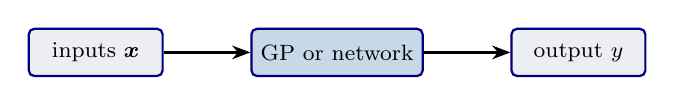
\begin{tikzpicture}[
    mlstep/.style={rectangle, draw=uzhblue, fill=uzhgreylight,
        minimum width=1.7cm, minimum height=0.6cm, font=\footnotesize,
        rounded corners=2pt, thick},
    >=Stealth
]
\node[mlstep] (input) {inputs $\x$};
\node[mlstep, right=1.1cm of input, fill=softblue!30] (dnn) {GP or network};
\node[mlstep, right=1.1cm of dnn] (output) {output $y$};
\draw[->, thick] (input) -- (dnn);
\draw[->, thick] (dnn) -- (output);
\end{tikzpicture}
\end{center}
\vspace{2pt}
{\footnotesize A table has one entry per grid point and dies of the curse of dimensionality. A fitted function is \emphc{continuous}, \emphc{differentiable}, and its cost grows with the complexity of $f$, not with $n_g^{d}$. Which function to fit is Part III.}
\end{column}
\end{columns}
\end{frame}

\begin{frame}{Building One, in Four Steps}
\small
\begin{enumerate}\itemsep3pt
  \item \textbf{Design.} Choose inputs $\x_i$, $i = 1,\dots,N$, spread over the box: uniform, Latin hypercube, Sobol' sequence, or (Part III) one at a time where the surrogate is least sure.
  \item \textbf{Label.} Evaluate the expensive model: $y_i = f(\x_i)$. \emphc{This is the step that costs money}, and it happens once.
  \item \textbf{Fit.} A Gaussian process (closed form) or a network (minimize $\frac1N\sum_i |\surr(\x_i) - y_i|^2$).
  \item \textbf{Validate.} Fresh labels the fit never saw: mean \emph{and} maximum error over the box, not a training loss.
\end{enumerate}

\vspace{0.2cm}
\begin{block}{Parameters as inputs}
Do not build one surrogate per parameter vector. Put the parameters $\str$ into $\x$ alongside the states, so that one fit answers for every $\str$ in the box. Session 7 estimates $\str$ by moving along that axis of one surrogate; Chen, Didisheim \& Scheidegger (2026) call them \emph{pseudo-states}.
\end{block}
\end{frame}

\begin{frame}{One Built on the Brock--Mirman Model}
\small
\vspace{-0.1cm}
\textbf{The expensive model:} the stochastic Brock--Mirman economy of Session 2 at a given $(\beta, \varrho)$, solved by a reference method (endogenous grid, cubic splines, Euler errors below $10^{-6}$), about 1.7 s per solve. \textbf{Quantity of interest:} the mean capital stock and the mean investment share along a 2{,}000-period simulation, $q(\beta, \varrho)$.

\vspace{0.1cm}
\begin{center}
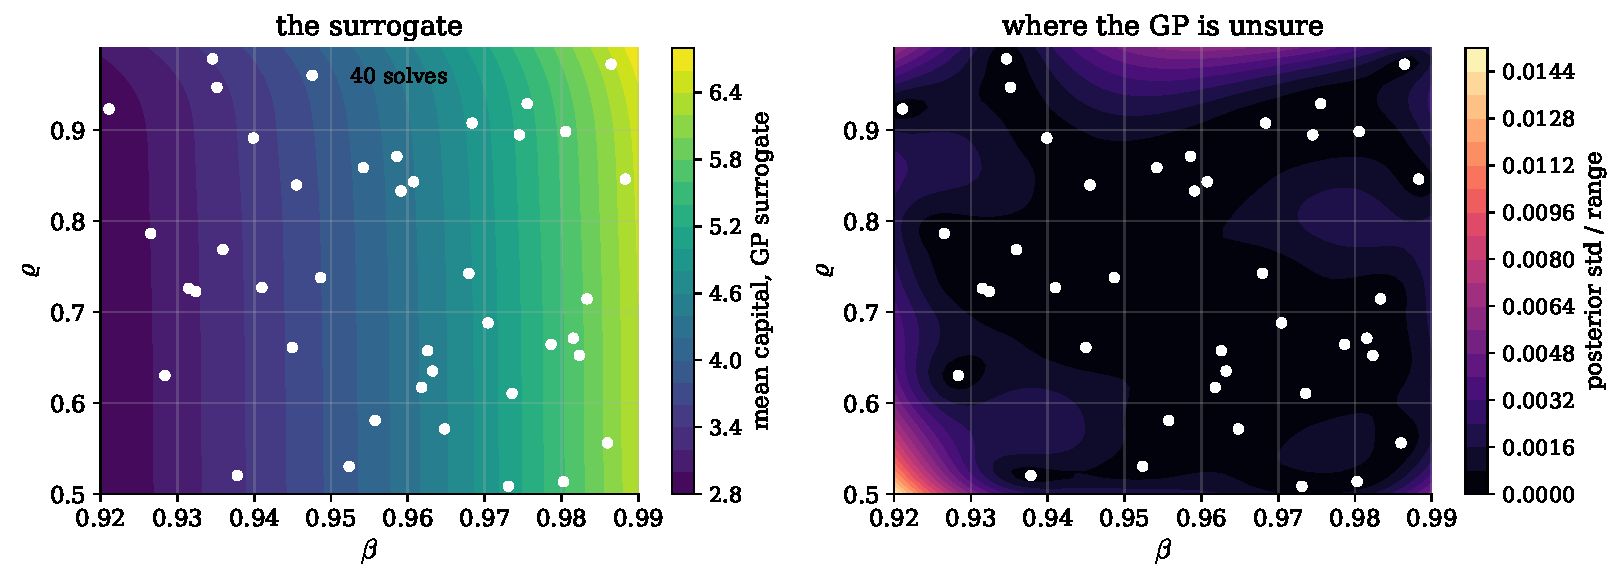
\includegraphics[width=0.98\linewidth]{figures/surrogate_primer_surface.pdf}
\end{center}
\vspace{-0.2cm}
{\footnotesize Notebook \texttt{06\_01}, stored teaching run. Left: the GP surrogate's mean capital over the box from \emphc{40 solves} (white dots), where a $30 \times 30$ grid would have cost 25 minutes. Middle: the GP's posterior standard deviation, largest away from the design. Right: on 60 fresh solves, the GP's error against the network's, both fit to the same 40 labels.}
\end{frame}

\begin{frame}{Two Kinds of Surrogate}
\small
\begin{columns}[T]
\column{0.48\textwidth}
\textbf{Labelled: a regression of $f$}
\begin{itemize}\itemsep2pt
  \item Inputs and outputs from the expensive solver
  \item Any approximator: GP, network, polynomial
  \item Summarizes what the model implies ($q$, moments, welfare)
  \item Cost $=$ number of solves
\end{itemize}
\vspace{0.1cm}
{\footnotesize This session: \texttt{06\_01}, \texttt{06\_02}.}

\column{0.48\textwidth}
\textbf{Trained on the equations: the solution itself}
\begin{itemize}\itemsep2pt
  \item A policy network $(\text{state}, \str) \mapsto$ decision
  \item Loss $=$ the Euler residual at sampled states, as in the DEQNs of Day 1
  \item No solver, no labels; $\str$ is one more input
  \item Cost $=$ training once
\end{itemize}
\vspace{0.1cm}
{\footnotesize Session 7: \texttt{07\_01}, \texttt{07\_02}, where the surrogate is simulated inside the estimator.}
\end{columns}

\vspace{0.3cm}
\begin{alertblock}{Same validation for both}
Compare with a reference solution at several $\str$, on the states the model actually visits. The Euler residual is a training loss, not an accuracy measure.
\end{alertblock}
\end{frame}

% ============================================================================
% PART II: GAUSSIAN PROCESSES
% ============================================================================

\begin{frame}{}
\begin{center}
{\Huge \textcolor{uzhblue}{Part II}}\\[0.8em]
{\LARGE Gaussian-Process Regression}
\end{center}
\end{frame}

% --- Conditioning is regression ---
\begin{frame}{Conditioning Is Regression}
\begin{columns}[T]
\column{0.48\textwidth}
\textbf{Joint:}
\[
\begin{pmatrix} x_1 \\ x_2 \end{pmatrix} \sim
\mathcal{N}\!\left(
\begin{pmatrix} \mu_1 \\ \mu_2 \end{pmatrix},
\begin{pmatrix} \Sigma_{11} & \Sigma_{12} \\ \Sigma_{21} & \Sigma_{22}\end{pmatrix}
\right)
\]

\vspace{0.25cm}
\textbf{Conditional:}
\begin{align*}
\mu_{1|2} &= \mu_1 + \Sigma_{12}\Sigma_{22}^{-1}(x_2 - \mu_2)\\
\Sigma_{1|2} &= \Sigma_{11} - \Sigma_{12}\Sigma_{22}^{-1}\Sigma_{21}
\end{align*}

\vspace{0.15cm}
\emphc{These two lines are the entire engine of GP regression.} Everything that follows is bookkeeping about how to build $\Sigma$.

\column{0.50\textwidth}
\begin{center}
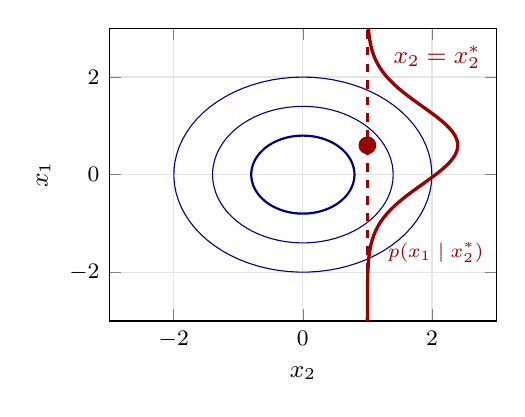
\begin{tikzpicture}
\begin{axis}[
    width=6.5cm, height=5.3cm,
    xlabel={$x_2$}, ylabel={$x_1$},
    xmin=-3, xmax=3, ymin=-3, ymax=3,
    grid=major, grid style={gray!20},
    every axis plot/.append style={no markers},
]
\addplot[uzhblue, thick, domain=0:360, samples=80]
    ({0.8*(0.894*cos(x) - 0.447*sin(x))}, {0.8*(0.447*cos(x) + 0.894*sin(x))});
\addplot[uzhblue, domain=0:360, samples=80]
    ({1.4*(0.894*cos(x) - 0.447*sin(x))}, {1.4*(0.447*cos(x) + 0.894*sin(x))});
\addplot[uzhblue, thin, domain=0:360, samples=80]
    ({2.0*(0.894*cos(x) - 0.447*sin(x))}, {2.0*(0.447*cos(x) + 0.894*sin(x))});
\draw[harvardcrimson, very thick, dashed] (axis cs:1,-3) -- (axis cs:1,3);
\node[font=\small, harvardcrimson, anchor=north east] at (axis cs:2.9,2.85) {$x_2 = x_2^*$};
\addplot[harvardcrimson, very thick, domain=-3:3, samples=80]
    ({1 + 1.4*exp(-(x-0.6)^2/(2*0.64))}, {x});
\node[font=\scriptsize, harvardcrimson, anchor=east, inner sep=1pt] at (axis cs:2.85,-1.6) {$p(x_1 \mid x_2^*)$};
\addplot[only marks, mark=*, mark size=3pt, harvardcrimson] coordinates {(1,0.6)};
\end{axis}
\end{tikzpicture}
\end{center}
{\small Slicing the joint at $x_2 = x_2^*$ leaves a 1D Gaussian: a prediction \emph{and} an error bar.}
\end{columns}
\end{frame}

% --- From observations to interpolation ---
\begin{frame}{From Observations to Interpolation}
\vspace{-0.2cm}
\begin{columns}[T]
\column{0.36\textwidth}
\begin{center}
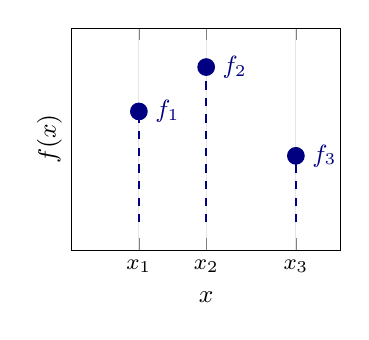
\begin{tikzpicture}
\begin{axis}[
    width=5.0cm, height=4.4cm,
    xlabel={$x$}, ylabel={$f(x)$},
    xmin=-0.5, xmax=5.5, ymin=-0.5, ymax=3.5,
    grid=major, grid style={gray!20},
    xtick={1,2.5,4.5}, xticklabels={$x_1$,$x_2$,$x_3$},
    ytick=\empty,
    every axis plot/.append style={no markers},
]
\addplot[uzhblue, thick, dashed] coordinates {(1,0) (1,2.0)};
\addplot[uzhblue, thick, dashed] coordinates {(2.5,0) (2.5,2.8)};
\addplot[uzhblue, thick, dashed] coordinates {(4.5,0) (4.5,1.2)};
\addplot[only marks, mark=*, mark size=3pt, uzhblue] coordinates {(1,2.0) (2.5,2.8) (4.5,1.2)};
\node[font=\small, uzhblue, anchor=west] at (axis cs:1.15,2.0) {$f_1$};
\node[font=\small, uzhblue, anchor=west] at (axis cs:2.65,2.8) {$f_2$};
\node[font=\small, uzhblue, anchor=west] at (axis cs:4.65,1.2) {$f_3$};
\end{axis}
\end{tikzpicture}
\end{center}
\column{0.58\textwidth}
\textbf{Assume} the function values are jointly Gaussian:
\vspace{-0.2cm}
{\small
\[
\begin{pmatrix} f_1 \\ f_2 \\ f_3 \end{pmatrix} \sim
\mathcal{N}\!\left(\bm{0},\;
\begin{pmatrix} K_{11} & K_{12} & K_{13} \\ K_{21} & K_{22} & K_{23} \\ K_{31} & K_{32} & K_{33}\end{pmatrix}\right)
\]
}

\vspace{-0.1cm}
\emphc{Nearby points should be more correlated than distant ones.} With a squared-exponential kernel and $\ell = 2$:
\[
K = \begin{pmatrix} 1.00 & 0.76 & 0.22 \\ 0.76 & 1.00 & 0.61 \\ 0.22 & 0.61 & 1.00 \end{pmatrix}
\]

\vspace{0.1cm}
Build the covariance from a \emphc{kernel}, $K_{ij} = k(x_i,x_j)$. Conditioning on the observed $f_i$ then predicts everywhere else.
\end{columns}
\end{frame}

% --- GP definition ---
\begin{frame}{A Gaussian Process: A Distribution over Functions}
\begin{block}{Definition}
A \emphc{Gaussian process} is a collection of random variables, any finite subset of which is jointly Gaussian:
\[
f(\x) \sim \mathcal{GP}\bigl(\mu(\x),\; k(\x,\x')\bigr).
\]
\end{block}

\begin{itemize}\itemsep2pt
  \item \textbf{Mean function} $\mu(\x) = \E{f(\x)}$, almost always $0$ after centering the data.
  \item \textbf{Covariance function} $k(\x,\x') = \E{(f(\x) - \mu(\x))(f(\x') - \mu(\x'))}$, where all the modeling lives.
\end{itemize}

\vspace{0.2cm}
\begin{center}
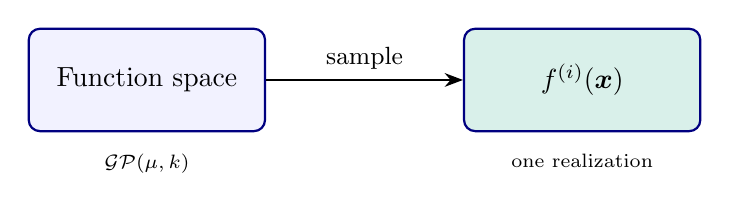
\begin{tikzpicture}[>=Stealth]
\node[draw=uzhblue, thick, rounded corners, fill=blue!5,
      minimum width=3cm, minimum height=1.3cm] (fspace) {Function space};
\node[right=2.5cm of fspace, draw=uzhblue, thick, rounded corners, fill=softgreen!15,
      minimum width=3cm, minimum height=1.3cm] (sample) {$f^{(i)}(\x)$};
\draw[->, thick] (fspace) -- node[above, font=\small] {sample} (sample);
\node[below=0.15cm of fspace, font=\scriptsize] {$\mathcal{GP}(\mu, k)$};
\node[below=0.15cm of sample, font=\scriptsize] {one realization};
\end{tikzpicture}
\end{center}
\end{frame}

% --- Kernels ---
\begin{frame}{Kernels: Where the Prior Lives}
\vspace{-0.1cm}
\begin{columns}[T]
\column{0.5\textwidth}
\begin{center}
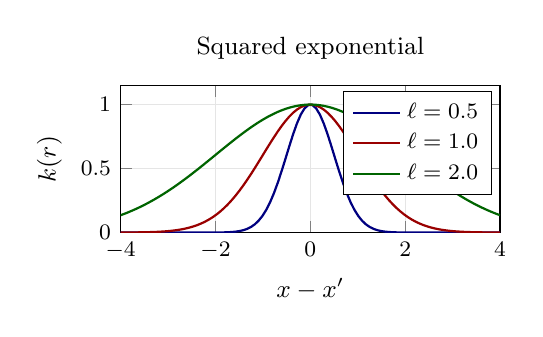
\begin{tikzpicture}
\begin{axis}[
    width=6.4cm, height=3.45cm,
    xlabel={$x - x'$}, ylabel={$k(r)$},
    xmin=-4, xmax=4, ymin=0, ymax=1.15,
    title={Squared exponential},
    legend style={at={(0.98,0.96)}, anchor=north east},
    grid=major, grid style={gray!20},
    every axis plot/.append style={thick, no markers},
]
\addplot[uzhblue, domain=-4:4, samples=100] {exp(-x^2/(2*0.5^2))};
\addlegendentry{$\ell = 0.5$}
\addplot[harvardcrimson, domain=-4:4, samples=100] {exp(-x^2/(2*1.0^2))};
\addlegendentry{$\ell = 1.0$}
\addplot[darkgreen, domain=-4:4, samples=100] {exp(-x^2/(2*2.0^2))};
\addlegendentry{$\ell = 2.0$}
\end{axis}
\end{tikzpicture}
\end{center}
{\footnotesize $k_{\mathrm{SE}}(r) = \sigma_f^2 \exp(-r^2/2\ell^2)$. Larger $\ell$ $\Rightarrow$ smoother; samples are \emphc{infinitely differentiable}, often too optimistic.}
\column{0.5\textwidth}
\begin{center}
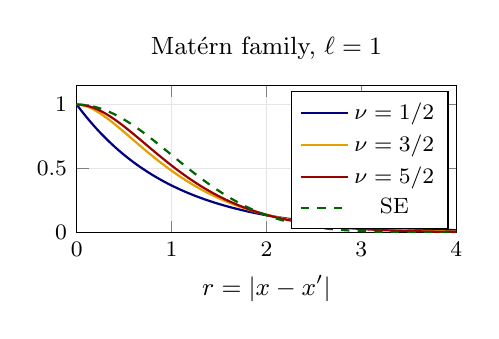
\begin{tikzpicture}
\begin{axis}[
    width=6.4cm, height=3.45cm,
    xlabel={$r = |x - x'|$},
    xmin=0, xmax=4, ymin=0, ymax=1.15,
    title={Mat\'ern family, $\ell = 1$},
    legend style={at={(0.98,0.96)}, anchor=north east},
    grid=major, grid style={gray!20},
    every axis plot/.append style={thick, no markers},
]
\addplot[uzhblue, domain=0:4, samples=200] {exp(-x)};
\addlegendentry{$\nu = 1/2$}
\addplot[softorange, domain=0:4, samples=200] {(1 + sqrt(3)*x)*exp(-sqrt(3)*x)};
\addlegendentry{$\nu = 3/2$}
\addplot[harvardcrimson, domain=0:4, samples=200] {(1 + sqrt(5)*x + 5*x^2/3)*exp(-sqrt(5)*x)};
\addlegendentry{$\nu = 5/2$}
\addplot[darkgreen, dashed, domain=0:4, samples=200] {exp(-x^2/2)};
\addlegendentry{SE}
\end{axis}
\end{tikzpicture}
\end{center}
{\footnotesize $\nu$ sets differentiability: samples are $\lceil \nu \rceil - 1$ times differentiable. \emphc{$\nu = 5/2$ or $3/2$ is the sane default} for value and policy functions.}
\end{columns}

\vspace{0.1cm}
{\footnotesize Choosing the kernel is not a technicality: it \emph{is} the model. Assume more smoothness than the truth has, and the GP interpolates confidently straight through a kink.}
\end{frame}

% --- Posterior ---
\begin{frame}{GP Regression: The Posterior in Two Lines}
\textbf{Joint distribution of training values $\bm f$ and test values $\bm f_*$:}
\[
\begin{pmatrix} \bm f \\ \bm f_* \end{pmatrix} \sim
\mathcal{N}\!\left(\bm 0,\;
\begin{pmatrix} K & K_* \\ K_*^\top & K_{**} \end{pmatrix}\right),
\qquad K_{ij} = k(\x_i, \x_j).
\]

\textbf{Condition on what you observed}: the two lines from three slides ago:
\begin{align*}
\bm\mu_{*|\mathcal{D}} &= K_*^\top K^{-1} \bm f\\
\Sigma_{*|\mathcal{D}} &= K_{**} - K_*^\top K^{-1} K_*
\end{align*}

\vspace{0.15cm}
\begin{alertblock}{Read the variance line carefully}
\begin{itemize}\itemsep1pt
  \item Near the data: $K_*^\top K^{-1} K_* \approx K_{**}$, so the variance \emphc{collapses}.
  \item Far from the data: $K_*^\top K^{-1} K_* \approx 0$, so the variance \emphc{reverts to the prior}.
\end{itemize}
\vspace{2pt}
Note what this means: the GP \emph{knows it is extrapolating}, and says so, without ever seeing the true function out there. No trained network does this by default.
\end{alertblock}
\end{frame}

% --- Noise ---
\begin{frame}{Noise, the Nugget, and Numerical Stability}
\small
\textbf{Observation model.} If labels carry noise, $y = f(\x) + \varepsilon$ with $\varepsilon \sim \mathcal{N}(0,\sigma_y^2)$, then $\mathrm{cov}[y_p, y_q] = k(\x_p,\x_q) + \sigma_y^2 \delta_{pq}$, so everywhere replace $K$ by $K_y = K + \sigma_y^2 I$:
\[
\bar f_* = \bm k_*^\top (K + \sigma_y^2 I)^{-1} \bm y,
\qquad
\sigma_*^2 = k(\x_*,\x_*) - \bm k_*^\top (K + \sigma_y^2 I)^{-1} \bm k_* .
\]

\vspace{0.2cm}
\begin{columns}[T]
\column{0.47\textwidth}
\textbf{Noiseless} ($\sigma_y^2 = 0$)
\begin{itemize}\itemsep1pt
  \item Interpolates the training points exactly
  \item Variance is zero at training inputs
  \item Needs $K$ strictly positive definite
\end{itemize}
\column{0.5\textwidth}
\textbf{Noisy} ($\sigma_y^2 > 0$)
\begin{itemize}\itemsep1pt
  \item Smooths through the training points
  \item Variance positive everywhere
  \item Much better conditioned
\end{itemize}
\end{columns}

\vspace{0.25cm}
\begin{block}{In practice}
Even for a ``noiseless'' surrogate, add a jitter of $\sigma_y^2 \sim 10^{-6}$. \emphc{And be honest about whether it really is noiseless}: if the labels came from a Monte Carlo simulation or an iterative solver stopped at a tolerance, they carry noise, and pretending otherwise makes the Cholesky factorization fail before it makes the statistics wrong.
\end{block}
\end{frame}

% --- Length scale ---
\begin{frame}{Getting the Length Scale Wrong}
\begin{center}
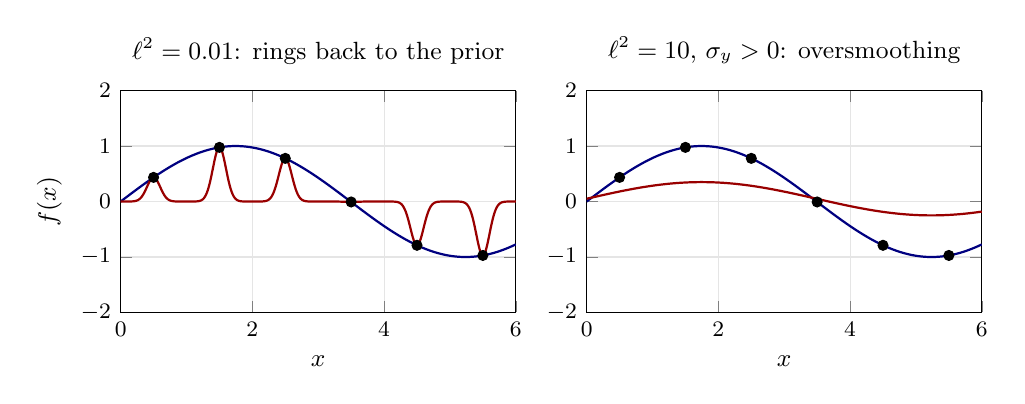
\begin{tikzpicture}
\begin{axis}[
    name=p1,
    width=6.6cm, height=4.4cm,
    title={$\ell^2 = 0.01$: rings back to the prior},
    xlabel={$x$}, ylabel={$f(x)$},
    xmin=0, xmax=6, ymin=-2, ymax=2,
    grid=major, grid style={gray!20},
    every axis plot/.append style={no markers},
]
\addplot[uzhblue, thick, domain=0:6, samples=200] {sin(deg(0.9*x))};
\addplot[harvardcrimson, thick, domain=0:6, samples=400]
    {0.435*exp(-(x-0.5)^2/0.02) + 0.976*exp(-(x-1.5)^2/0.02)
   + 0.778*exp(-(x-2.5)^2/0.02) - 0.008*exp(-(x-3.5)^2/0.02)
   - 0.789*exp(-(x-4.5)^2/0.02) - 0.972*exp(-(x-5.5)^2/0.02)};
\addplot[only marks, mark=*, mark size=1.8pt, black] coordinates
    {(0.5,0.435) (1.5,0.976) (2.5,0.778) (3.5,-0.008) (4.5,-0.789) (5.5,-0.972)};
\end{axis}

\begin{axis}[
    at={(p1.east)}, anchor=west, xshift=0.9cm,
    width=6.6cm, height=4.4cm,
    title={$\ell^2 = 10$, $\sigma_y > 0$: oversmoothing},
    xlabel={$x$},
    xmin=0, xmax=6, ymin=-2, ymax=2,
    grid=major, grid style={gray!20},
    every axis plot/.append style={no markers},
]
\addplot[uzhblue, thick, domain=0:6, samples=200] {sin(deg(0.9*x))};
\addplot[harvardcrimson, thick, domain=0:6, samples=200] {0.30*sin(deg(0.9*x)) + 0.05};
\addplot[only marks, mark=*, mark size=1.8pt, black] coordinates
    {(0.5,0.435) (1.5,0.976) (2.5,0.778) (3.5,-0.008) (4.5,-0.789) (5.5,-0.972)};
\end{axis}
\end{tikzpicture}
\end{center}

\vspace{0.1cm}
\small
\begin{columns}[T]
\column{0.48\textwidth}
\textbf{Too short.} The GP interpolates every point exactly and then \emphc{falls back to the prior mean in between}. Perfect training fit, useless predictions, and the credible band (previous slide) balloons in exactly those gaps.
\column{0.48\textwidth}
\textbf{Too long.} The posterior mean flattens and no longer passes through the data. The band is narrow and \emphc{confidently wrong}, which is the more dangerous failure of the two.
\end{columns}
\end{frame}

% --- Hyperparameters ---
\begin{frame}{Learning the Hyperparameters, and a Free Diagnostic}
\small
\begin{block}{Marginal likelihood: how $\ell$, $\sigma_f$, $\sigma_y$ get chosen}
\vspace{-6pt}
\[
\log p(\bm y \mid X) =
\underbrace{-\tfrac{1}{2}\bm y^\top K_y^{-1} \bm y}_{\text{data fit}}
\underbrace{-\tfrac{1}{2}\log|K_y|}_{\text{complexity penalty}}
\underbrace{-\tfrac{N}{2}\log(2\pi)}_{\text{constant}}
\]
\vspace{-8pt}

The two terms pull against each other: \emphc{an automatic Occam's razor}, with closed-form gradients and no validation split spent. Optimize with restarts; it is multimodal.
\end{block}

\vspace{0.08cm}
\begin{block}{Leave-one-out, for free}
\vspace{-6pt}
\[
\mu_{-i}(\x_i) - y_i = -\frac{[K_y^{-1}\bm y]_i}{[K_y^{-1}]_{ii}},
\qquad
\sigma^2_{-i}(\x_i) = \frac{1}{[K_y^{-1}]_{ii}} .
\]
\vspace{-8pt}

These need $\mathrm{diag}(K_y^{-1})$, so \emph{all $N$} leave-one-out residuals cost one further $\mathcal{O}(N^3)$ solve, the same order you already paid, and \emphc{no refitting and no held-out data}. Doing $N$ honest refits would be $\mathcal{O}(N^4)$. \emphc{This is the number to report for a surrogate.}
\end{block}

\vspace{0.1cm}
{\footnotesize Closed form: Rasmussen \& Williams (2006), \S\,5.4.2, in \texttt{../readings}.}
\end{frame}

% --- Code ---
\begin{frame}[fragile]{GP Regression in Fifteen Lines}
\begin{lstlisting}[basicstyle=\scriptsize\ttfamily]
import numpy as np
from scipy.linalg import cho_factor, cho_solve

def kernel(X1, X2, l=1.0, sf=1.0):
    sq = np.sum(X1**2, 1).reshape(-1, 1) \
         + np.sum(X2**2, 1) - 2 * X1 @ X2.T
    return sf**2 * np.exp(-0.5 * sq / l**2)

K = kernel(X_tr, X_tr) + 1e-8 * np.eye(N)   # jitter
L, low = cho_factor(K, lower=True)          # O(N^3), once
alpha  = cho_solve((L, low), y_tr)          # the weights

Ks  = kernel(X_tr, X_te)
mu  = Ks.T @ alpha                          # posterior mean
v   = cho_solve((L, low), Ks)
var = kernel(X_te, X_te) - Ks.T @ v         # posterior variance
\end{lstlisting}

\vspace{0.1cm}
{\footnotesize No training loop, no learning rate, no architecture: the whole model is the kernel and one Cholesky factorization. Compare Algorithm 2.1 in Rasmussen \& Williams (2006); notebook \texttt{06\_02} builds this and checks it against \texttt{scikit-learn}.}
\end{frame}


\begin{frame}{Prediction and Credible Bands}
\begin{center}
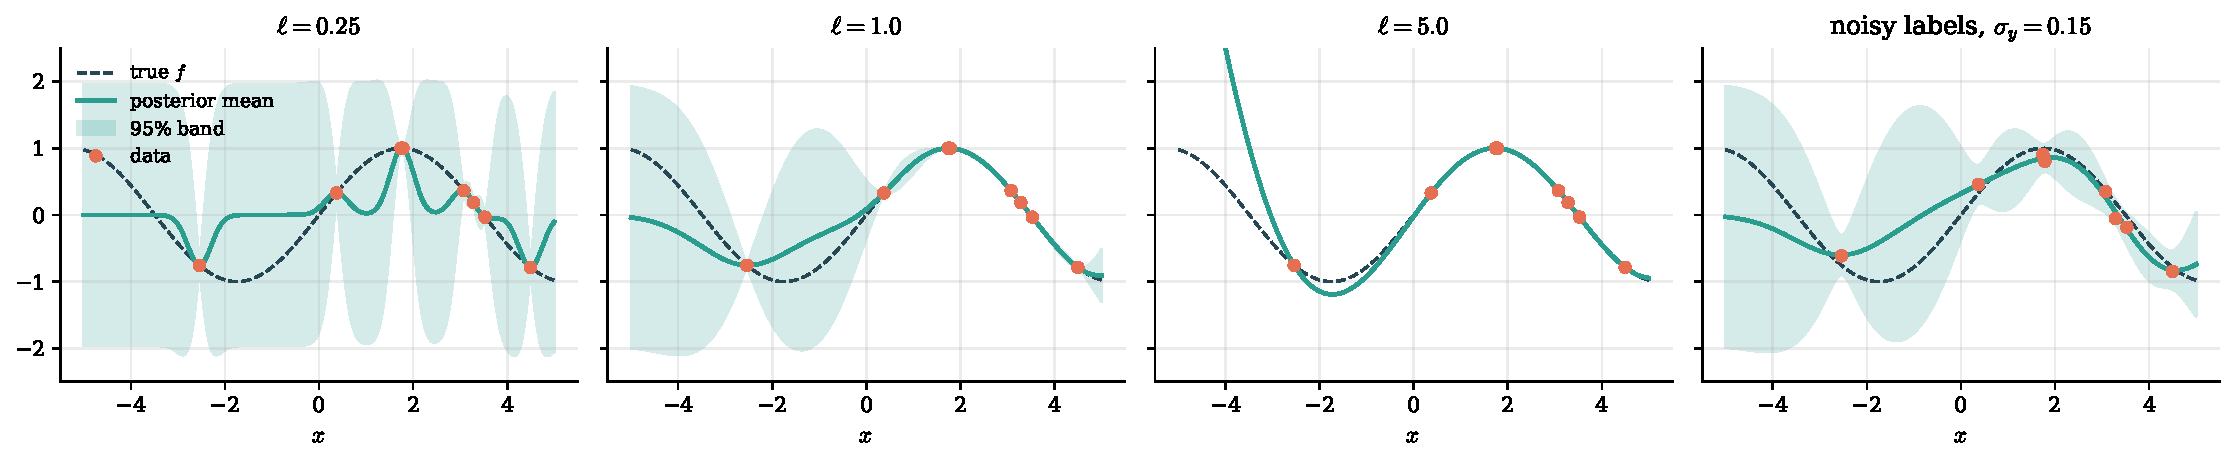
\includegraphics[width=0.92\linewidth]{figures/gp_length_scale.pdf}
\end{center}
\vspace{-0.2cm}
{\footnotesize Notebook \texttt{06\_02}, eight exact observations of $\sin(0.9x)$, squared-exponential kernel. The band pinches shut at each observation and opens between them. Left to right: length scale too short (returns to the prior mean between points), right, too long (confidently wrong), and noisy labels with $\sigma_y = 0.15$ (smooths through the points).}
\end{frame}

% ============================================================================
% PART III: GP OR NETWORK
% ============================================================================

\begin{frame}{}
\begin{center}
{\Huge \textcolor{uzhblue}{Part III}}\\[0.8em]
{\LARGE GP or Network?}
\end{center}
\end{frame}

\begin{frame}{The Same Task, Both Surrogates}
\begin{center}
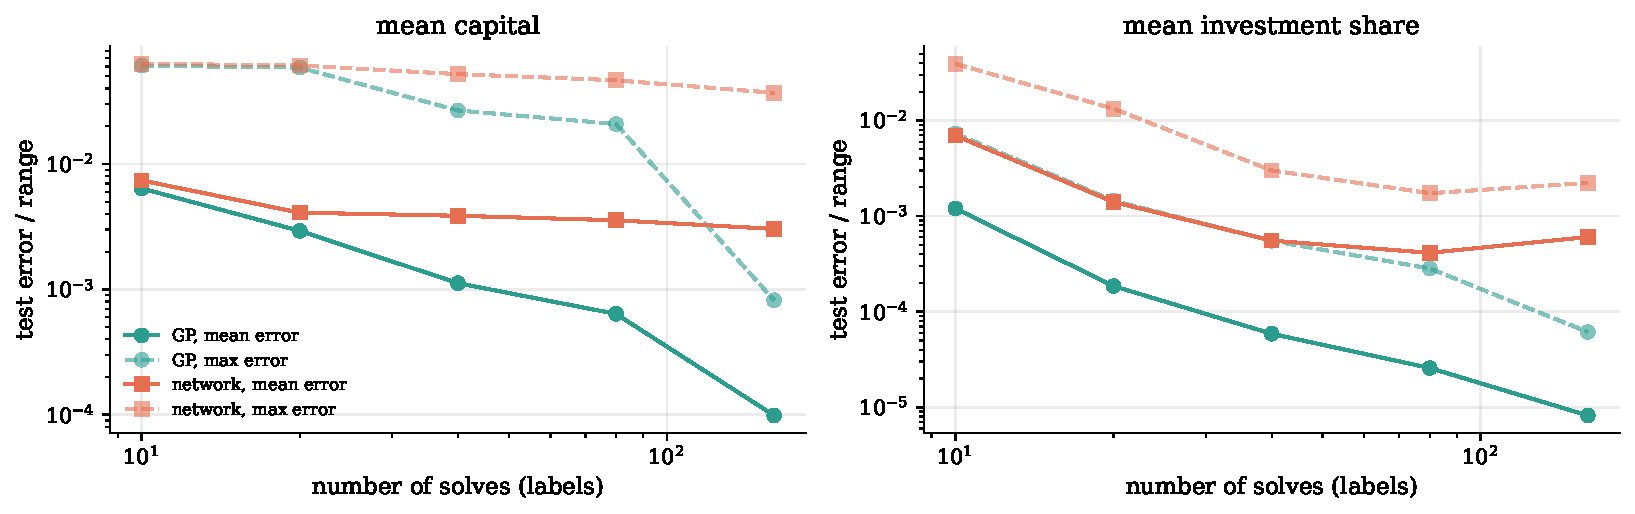
\includegraphics[width=0.9\linewidth]{figures/surrogate_primer_error_vs_n.pdf}
\end{center}
\vspace{-0.2cm}
{\footnotesize Notebook \texttt{06\_01}: the same labels, the same 60 test solves, error relative to the range of the quantity. GP: Matérn 5/2, one length scale per input, hyperparameters by marginal likelihood. Network: $2\times32$ tanh, Adam, 3{,}000 epochs. For the mean capital stock the GP's mean error is $6.4\cdot10^{-3}$ at $N=10$ and $9.9\cdot10^{-5}$ at $N=160$, the network's $7.4\cdot10^{-3}$ and $3.0\cdot10^{-3}$; the GP is ahead at every budget from $N=10$ on. The GP's 95\% band covered the truth at 97\% and 98\% (mean capital, investment share) at $N=160$ of the test points.}
\end{frame}

\begin{frame}{The Decision Rule Is the Cost of a Label}
\begin{center}
\scriptsize
\setlength{\tabcolsep}{4pt}
\begin{tabular}{l l l}
\toprule
\textbf{Criterion} & \textbf{Gaussian process} & \textbf{Network} \\
\midrule
Uncertainty & \yes posterior variance, calibrated & \no needs ensembles \\
Hyperparameters & \yes marginal likelihood, closed-form gradient & \mixed search (Session 3) \\
Fitting & \yes one Cholesky factorization & \mixed SGD, epochs, seeds \\
Scaling in $N$ & \no $\mathcal{O}(N^3)$, practical limit ${\sim}10^4$ & \yes $\mathcal{O}(N)$ per epoch \\
Scaling in $d$ & \no degrades past $d \approx 10$ & \yes $d \gg 100$ \\
Few labels ($N < 100$) & \yes & \no \\
\bottomrule
\end{tabular}
\end{center}

\vspace{0.05cm}
\begin{alertblock}{In order}
\footnotesize
\begin{enumerate}\itemsep1pt
  \item \textbf{Price one label.} Seconds, or hours? Hours means $N$ will be small, and the $\mathcal{O}(N^3)$ never bites.
  \item \textbf{Count the inputs} after adding the parameters. Ten or fewer favours the GP.
  \item \textbf{Ask whether a decision rides on the surrogate.} If so, you need the error bar.
  \item \textbf{Labels cheap and $d$ large:} network. \textbf{Labels expensive and $d$ small:} GP. \textbf{Both:} a policy network solves the model, a GP maps its output to the quantity of interest.
\end{enumerate}
\end{alertblock}
\end{frame}

\begin{frame}{Active Learning, in One Frame}
\small
The posterior variance depends on the design, not on the labels, so it can be consulted \emph{before} paying for the next label: query where it is largest, refit, repeat.

\vspace{0.1cm}
\begin{center}

\includegraphics[width=0.9\linewidth]{figures/gp_active_learning.pdf}
\end{center}
\vspace{-0.2cm}
{\footnotesize Notebook \texttt{06\_02}, $|\sin(\pi x/2)|$ from two endpoints; the dotted line is the next query. On an interval this ends level with or behind a uniform design (mean absolute error 0.0923 against 0.0673 with 10 points), and it should: spreading out the variance and spreading out the points are the same thing there, and the uniform design does it in one step. It earns its keep where no space-filling design exists: irregular domains, unequal length scales, many dimensions. Scheidegger \& Bilionis (2019), in \texttt{../readings}, run this loop on economic models.}
\end{frame}

\begin{frame}{Finger Exercise: How Many Labels?}
\begin{flushright}\exercisepause{}\end{flushright}
\vspace{-0.35cm}
\begin{exampleblock}{The setting}
You must map a welfare objective over a \emphc{6-dimensional} policy box. One evaluation means simulating a stochastic OLG model, $\approx 4$ hours of wall-clock time. You have a 64-core machine and \emphc{two weeks}.
\end{exampleblock}

\vspace{0.4cm}
\begin{enumerate}\itemsep6pt
  \item Roughly how many evaluations can you afford?
  \item How many points per dimension would a tensor grid give you at that budget?
  \item Which approximator does that budget select, and why?
\end{enumerate}
\end{frame}

\begin{frame}{Solution: How Many Labels?}
\small
\begin{block}{1. The budget}
$14 \text{ days} \times 24 \text{ h} = 336$ h of wall-clock time; at 64 cores that is ${\sim}21{,}500$ core-hours, so about \emphc{5{,}000 evaluations} at 4 h each. Call it a few thousand, allowing for failures and re-runs.
\end{block}

\begin{block}{2. What a grid does with them}
$5{,}376^{1/6} \approx 4.2$ points per dimension. Four per axis will not resolve a curved welfare surface, and refining to a still-inadequate six costs $6^6 = 46{,}656$ evaluations $= 187{,}000$ core-hours, or \emphc{four months} on the same 64 cores.
\end{block}

\begin{block}{3. Which approximator}
A few thousand points is far too few to train a network well, and comfortably inside the $\mathcal{O}(N^3)$ range of an exact GP. \emphc{Choose the GP}, and since every point is precious, do not place them on a grid at all: let the posterior variance choose them.
\end{block}
\end{frame}

\begin{frame}{Hands-On: What to Run}
\small
Notebooks in \texttt{day2/code/06\_surrogates\_and\_gps}, CPU-only. Both ship with the teaching preset stored; in class set \texttt{RUN\_MODE = "smoke"} first.

\vspace{0.2cm}
\begin{itemize}\itemsep5pt
  \item \textbf{Surrogates, the idea} \emph{(6 min)}. Time one solve of the Brock--Mirman model; label a Latin-hypercube design; fit a GP and a network to the same labels; watch both errors fall with the number of solves, and check whether the GP's band is calibrated. \hfill{\footnotesize\texttt{06\_01}}
  \item \textbf{GP regression} \emph{(28 s)}. The kernel and prior samples; the posterior in two lines, checked against scikit-learn; length scale and noise; Matérn against squared-exponential on a kink; two inputs with one length scale each; the active-learning loop. \hfill{\footnotesize\texttt{06\_02}}
\end{itemize}

\vspace{0.3cm}
\begin{block}{Next session}
The surrogate becomes the model's own policy, with $\varrho$ and then $(\beta, \varrho)$ as inputs, and is simulated inside an SMM estimator.
\end{block}
\end{frame}

\begin{frame}{}
\begin{columns}[c]
\column{0.42\textwidth}
\begin{center}
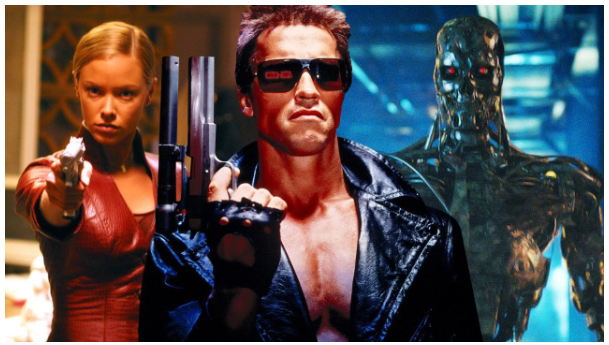
\includegraphics[width=0.8\linewidth]{figures/quest.png}
\end{center}
\column{0.55\textwidth}
{\LARGE \textcolor{uzhblue}{Questions?}}

\vspace{0.5cm}
{\small
\textbf{Simon Scheidegger}\\
HEC, University of Lausanne\\[4pt]
\href{mailto:simon.scheidegger@unil.ch}{simon.scheidegger@unil.ch}~~$\cdot$~~\href{https://sischei.github.io}{sischei.github.io}
}

\vspace{0.5cm}
{\footnotesize
\textbf{Next up, Session 7:} \emph{Structural estimation via the simulated method of moments.}
}

\vspace{0.4cm}
{\footnotesize
\textbf{Materials:}\\ \href{https://github.com/sischei/deep_learning_padova_0926}{github.com/sischei/deep\_learning\_padova\_0926}
}
\end{columns}
\end{frame}

\end{document}
